\section{Designing the Playing Field}
\label{sec:designing_playing_field}
As stated in the requirements section, the game will be displayed as a 2D environment instead of 3D, since the focus of this project is not on the graphical presentation of the game, but on the combination of engaging gameplay and education. However, there are still different approaches when designing the playing field. This section will focus on these approaches and argue why some solutions have been chosen over others. We will use our own game, where the player programs a cell to move around the environment to eliminate enemy cells as an example.

\subsection{Free Environment vs. Tile-styled}

When approaching the design of a 2D environment, it might be possible to design the layout as being free or limited.
In a free environment, the cell would be able to move in all 360$^{\circ}$.
This approach is seen in the game \textit{Osmos}, that is similar to our game without the programming aspect.
The player can move a cell freely in the 2D environment to eat smaller cell and each level has a specific objective.
However, the free environment approach would possibly increase the difficulty of programming the cell in contrast to a tile-styled approach to design.
The reader might imagine, that it is more difficult to program a cell to move in 360 different directions than in for example 4 or 6.
Note, that by tiles we do not mean traditional tiles, such as those used in \textit{Mahjong} and \textit{Domino}, but rather games were the playing field is made by the players at the beginning of game by laying tiles with different properties.
The tile-style is known from board games, such as \textit{The Settlers of Catan} and \textit{Hive}, where both board games use hexagonal tiles.
However, tiles may not be restricted to being hexagonal, but we will discuss this later in this section.\\

Using tiles would limit the available movements of each cell into $x$ number of directions, where $x$ denotes the amount of sides on a single tile. This limiting factor would make it easier for the player to program each cell, because for example $6$ movement options are much less than $360$. The question is then whether the tile-styled approach would limit the player too much, making the game less engaging and too easy. However, the same question can be applied to the free environment approach.\\

We have chosen to design the playing field as a tile-styled board game, since we do not think that the limitation of tiles makes the programming of the cells too easy. It might even increase the user base, by allowing less experienced player to program cells that have a chance to defeat more experienced players. This also effects the more experienced players, since, if multiplayer is implemented, the experienced players will then face more difficult cells. We judge, that the sense of achievement when having defeated a difficult opponent is greater than when the opponent is weak and easy to defeat.\\

However, as mentioned easier, tiles can have $x$ number of sides. The next subsection will focus on how to design the tiles in terms of number of sides on each tile and whether tiles should include different properties.

\subsection{Designing the Tiles - Polygons}

Polygons are closed $2$ dimensional object that have more than $2$ sides.
The smallest polygon in term of sides is therefore the triangle.
\textit{Bizingo} is a board game that use triangle tiles, but we have not been able to find other games.
It is far more common to see games that use either square or hexagonal tiles.
Therefore, they both have the appeal of being more recognizable to the user, thereby making the game easier to learn.
We will mainly discuss the pros and cons with square and hexagonal tiles.\\

\subsubsection{4 vs 6}

In terms of the players ability to move, square tiles would only allow for four movements, while hex tiles would allow for 6.
This might not seem as a big difference, however, if we want the game to be realistic or similar to something real, the more freedom we allow the user, the more real the game may seem.
This might seem as an argument for choosing the free environment approach, but we argue that it would be more difficult for the players to program into a free environment, and that the tile based approach would lead to more balanced games between players, if multiplayer is implemented.
Therefore, hex tiles describe more realistic movements.\\

Some may argue, that if 6 sided tiles are more realistic than 4 sided, then why not go further an use 8 or 10 sided tiles. Here we will argue, that 8 or 10 sided tiles do not fit well with each other, since there will be holes in the playing field. These holes does not appear when using 4 or 6 sided tiles. This means, that the amount of move in a 8 sided tile is also 4, not 8, see \autoref{fig:tiles_dif}.

\begin{figure}[h]
  \centering
    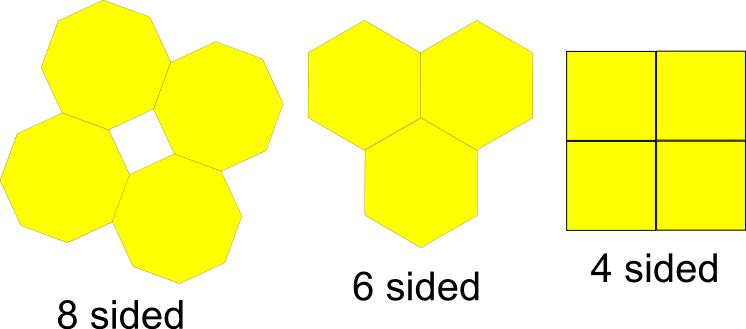
\includegraphics[width=0.6\textwidth]{img/8-6-4-sided-tiles.png}
  \caption{Difference between 8, 6, and 4 sided tiles}
  \label{fig:tiles_dif}
\end{figure}

In the end it came down to a design decision on the groups behalf between square and hexagon. There is little difference between the two, even though we have argued that hex allow more realistic movements. In the end we chose the hex tiles approach.



